\begin{minipage}{.35\textwidth}
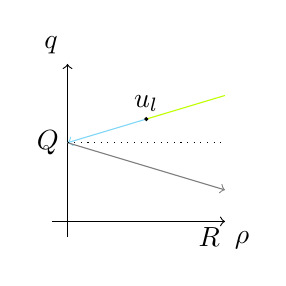
\begin{tikzpicture}
% coordinates
\draw[->] (0,-0.2) -- (0,2) node[anchor= south east] {$q$};
\draw[->] (-0.2,0) -- (2,0) node[anchor= north west] {$\rho$};
% rarefactions

\draw[lime] (1, 1.3) -- (2, 1.6) ;
\draw[<-][cyan!50] (0, 1) -- (1, 1.3) ;
\draw[->][black!50] (0, 1) -- (2, 0.4) ;
\draw[dotted] (0,1) -- (2, 1);
\filldraw[black] (1,1.3) circle (0.5pt) ;
\node at (1, 1.5) {$u_l$};
\node at (1.8, -0.2) {$R$};
\node at (-0.25, 1) {$Q$};
\end{tikzpicture}
\caption{Lax entropy for $q > Q$. \\ Rarefaction (blue) and \\shock (green).}
\label{Fig:LaxEntropy1CongestedPhase}
\end{minipage}
\quad \quad \quad \quad 
\begin{minipage}{.35\textwidth}
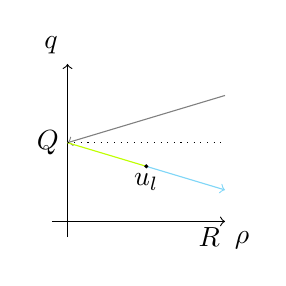
\begin{tikzpicture}
% coordinates
\draw[->] (0,-0.2) -- (0,2) node[anchor= south east] {$q$};
\draw[->] (-0.2,0) -- (2,0) node[anchor= north west] {$\rho$};
% rarefactions
\draw[<-][black!50] (0, 1) -- (2, 1.6) ;
\draw[->][cyan!50] (1,0.7) -- (2, 0.4) ;
\draw[-][lime] (0, 1) -- (1,0.7) ;
\draw[dotted] (0,1) -- (2, 1);
\filldraw[black] (1,0.7) circle (0.5pt) ;
\node at (1, 0.5) {$u_l$};
\node at (1.8, -0.2) {$R$};
\node at (-0.25, 1) {$Q$};
\end{tikzpicture}
\caption{Lax entropy for $q < Q$ \\ Rarefaction (blue) and \\shock (green).}
\label{Fig:LaxEntropy2CongestedPhase}
\end{minipage}